\chapter{Implementation/Tests}
\label{chap:Implementation}
\todo{integration tests explaining sequence diagrams}

In this chapter I will discuss some of the decisions I have made while
developing the system, and why I made that decision instead of going with
another implementation that was possible.

I will also cover some of the ways I have used the technologies that I chose in
the previous chapter, as well as how they are working together.

In the end I will get a bit into how I have tested the system throughout the
development process, both in regards to unit testing and integration testing.

\section{Entity framework}
\label{sec:Entity framework}
One of the things the entity framework brings is the "repository pattern", as
well as the "Unit of Work pattern". The idea behind those are described in
section~\ref{sec:Patterns}. I however have chosen to wrap them again, so that I
can reduce the dependency to a database implementation and ORM implementation,
in the outer most layer. 

The decision to wrap the implementations also allow me to mock the
implementations a bit easier in some cases when it comes to testing. 

Instead of having a controller call the entity implementations directly, I have
a set of interfaces in the DomainServices layer of the onion model, that I can
use for injection, these interfaces implement my personal implementations of
repositories, and allow me to customize the way I want to deal with the data. 

I have a generic repository, which is capable of doing the most common
operations, such as add a new model to the database, and getting them out again.
It also makes sure to set the right states of the model when I update a model,
and delete one. 

One thing that I use is the idea of telling the repository how I want it to
update the existing model via an action, which it takes as an argument. The
reason for that is it allows me to not update all the properties, but only the
ones that is relevant. Because I only update the relevant ones, if the User of
the program sends in changed data for a property they are not supposed to be
able to change, it will not be changed. 

The generic interface also allows me to implement a standardized way of dealing
with pagination, which is the idea of instead of pulling everything out of a
table, we order the entries, and return a subset of the data. 

This allows the user to ask for ex 10 entries in the table Users, and only get
the 10 entries they asked for. Because they are now not getting all the data
they need to be told how much data there is, and therefore we return the total
number of entries in the search, as well as the page size they got, and the page
they are looking at. The page number is used to set the first entry to the one
with $index = page number \cdot page size$. 

In the simple cases I let the controllers depend on the generic repository, as
there is no need to implement a special handling of cases where no special
update or create logic is needed. But for the cases where we need to link tables
together I have decided to make specific implementations, which themselves
depend on the generic repository, as the logic to save get and update can be
reused, there just needs to be added some more logic on to it. 

I don't have any saving logic in any of the repositories, because I want to be
able to make multiple repository calls in one go, and if any of them fails the
idea of unit of work should step in and make sure that none of the changes take
place. 

Because of this I have implemented a interface to handle the unit of work, with
the ability to call save changes, which all the controllers implement, and use
in the cases where data changes. 

The only place where I don't follow these setups is in the user controller, as
it uses the Identity framework for authentication and authorization, and it
brings its own user manager, which I need to use if I want the feature they
bring. The problem with this user manager is that it does not follow the unit of
work pattern, which means it saves every time I make a call that would update
the database. 

\section{Exception filters}
\label{sec:Exception filters}
To be able to return the appropriate response when something fails, I have
decided to throw appropriate exceptions, with messages of what went wrong in
case that is not obvious from the exception itself.

To help with this I have implemented an extention method for getting things out
of the database. If I want to get a single thing out, I would call
SingleOrDefault, but if I need the result to be something, and the defult value
therefore is not useful. For this I have implemented the extention function
SingleOrExcept, which just uses SingleOrDefault where if it returns null it
throws a NotFoundException.

To make the response appropriate in the controller I could go with different
approaches. The most basic way of dealing with this would be to catch the
exceptions, and return the right message to the client.

Another way to deal with this is to use filters, this is the way I have decided
to go with. For filters there are still multiple ways to do this, I could have
set the filter on a per method, per controller, or for the entire server.

The implementation of the filter would look like the one of
figure~\ref{fig:notfoundfilter} for all of the types, and since I need the
filters to apply to all the controllers I have gone with the cross project
solution. 

\begin{figure}
  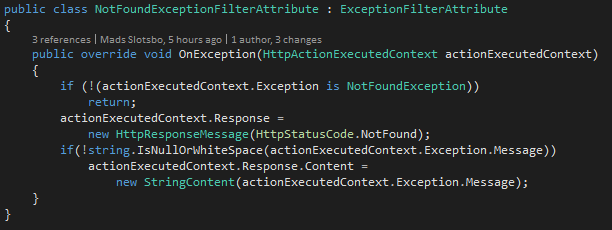
\includegraphics[width=\textwidth]{code/NotFoundExceptionFilterAttribute}
  \caption{NotFoundException filter}
  \label{fig:notfoundfilter}
\end{figure}

\section{Graph data calls}
\label{sec:Graph data calls}
For the data extraction I start by pulling the data out of the database, and
then send it to the method that will format it properly. The reason I do it like
this is that it allows me to use the method no matter where the data comes from. 

I make use of LINQ\footnote{Language-Integrated query} to manipulate the data
since it allows me to group by different keys, and filter away some of the data.

For the production graph, i have two calls, one for the production data, and one
for the goal data. The call for production data is the most interesting, in that
it needs to deal with spacing the earned money out over the period it spans in.

This also means that i had to make a filter that includes the opportunity as
long as it is within the range on the period.

\begin{figure}
  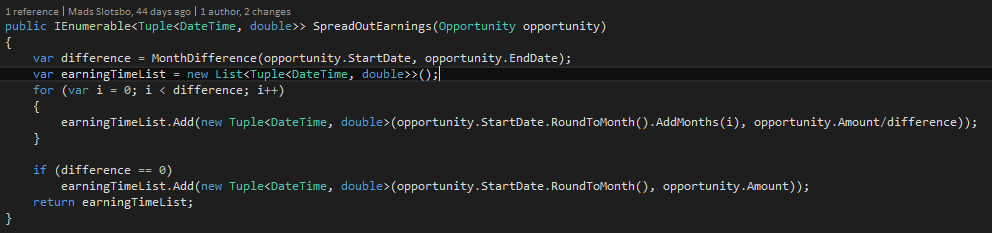
\includegraphics[width=\textwidth]{code/SpreadOutEarnings}
  \caption{SpreadOutEarnings implementation}
  \label{fig:spreadoutearnings}
\end{figure}

In figure~\ref{fig:spreadoutearnings} the implementation of the evening out of
the earnings is illustrated, as can be seen the implementation the result os a
list of tuples. The reason i use tuples here is that it allows me to assosiate
the earned value with the month it was earned.

When the list is returned I filter away the months that i don't need, based on
the filter, and match it up with a user.

In the end I map the result to a dictionary, with the users email as the key.
The reason I can do that is that the email is uniqueue, and I have grouped them
together ahead of time, to allow me to only have one dictionary entry per user,
containing a list of earnings per month.

\section{Unit tests}
\label{sec:unit_tests}

\section{Integration tests}
\label{sec:integration_tests}

\section{Chapter summary}
